% Ray tracing stereographic Hopf tori
% Generated from ../TECHNICAL_NOTE.md by ../scripts/build-latex.py.
% This file is standalone and can also be edited directly.
% Compile twice with pdflatex main.tex .
\documentclass[11pt,a4paper]{article}
\usepackage[T1]{fontenc}
\usepackage[utf8]{inputenc}
\usepackage{lmodern}
\usepackage[margin=24mm]{geometry}
\usepackage{amsmath,amssymb}
\usepackage{microtype}
\usepackage{xcolor}
\usepackage{booktabs,longtable,array,calc}
\usepackage{graphicx,caption,float,needspace}
\usepackage[section]{placeins}
\captionsetup{font=small,labelfont=bf,skip=8pt}
\providecommand{\pandocbounded}[1]{#1}
\usepackage{enumitem}
\usepackage{fancyvrb}
\usepackage{fancyhdr}
\usepackage{titlesec}
\usepackage{xurl}
\usepackage{hyperref}
\definecolor{ink}{HTML}{172D36}
\definecolor{accent}{HTML}{126B72}
\hypersetup{colorlinks=true,linkcolor=accent,urlcolor=accent,citecolor=accent,
  pdftitle={Ray tracing stereographic Hopf tori across the projection pole},
  pdfauthor={Tom Crosby},
  pdfsubject={Geometry, quartic intersections, and solid and shell optics in Hopf Observatory}}
\urlstyle{same}
\setlength{\parindent}{0pt}
\setlength{\parskip}{0.45em plus 0.15em minus 0.1em}
\setlength{\emergencystretch}{2em}
\setlength{\tabcolsep}{5pt}
\renewcommand{\arraystretch}{1.13}
\setlist{itemsep=0.35em,topsep=0.4em,leftmargin=*}
\providecommand{\tightlist}{\setlength{\itemsep}{0pt}\setlength{\parskip}{0pt}}
\titleformat{\section}{\large\sffamily\bfseries\color{ink}}{\thesection}{0.7em}{}
\titleformat{\subsection}{\normalsize\sffamily\bfseries\color{ink}}{\thesubsection}{0.7em}{}
\titlespacing*{\section}{0pt}{1.5em}{0.6em}
\titlespacing*{\subsection}{0pt}{1em}{0.4em}
\pagestyle{fancy}
\fancyhf{}
\fancyhead[L]{\small\sffamily\color{accent}Hopf Observatory}
\fancyhead[R]{\small\sffamily Technical note}
\fancyfoot[C]{\small\thepage}
\setlength{\headheight}{14pt}
\renewcommand{\headrulewidth}{0.3pt}
\clubpenalty=10000
\widowpenalty=10000
\displaywidowpenalty=10000
\begin{document}
\thispagestyle{plain}
{\sffamily\bfseries\color{ink}\LARGE Ray tracing stereographic Hopf tori\\across the projection pole\par}
\vspace{0.5em}
{\sffamily\large Geometry, quartic intersections, and solid and shell optics\par}
\vspace{0.5em}
{\sffamily Tom Crosby\par}
{\small\href{mailto:twcrosbynz@gmail.com}{twcrosbynz@gmail.com}\par}
\vspace{0.3em}
{\sffamily\small Hopf Observatory \enspace\textbar\enspace 21 November 2026 \enspace\textbar\enspace Technical note\par}
\vspace{0.4em}
{\color{accent}\rule{\linewidth}{0.8pt}}
\begin{abstract}
This note describes an interactive GPU ray tracer for stereographic
images of rotated Hopf tori, and derives everything it computes. The
tori are level sets of a rank-two quadratic form on the three-sphere. A
straight camera ray lifts to a circle on that sphere, so each
intersection is a root of a quartic in the ray parameter, with analytic
normals from the same form. Closest-point recentering and
near/reciprocal ray coordinates keep the quartic on bounded intervals
even when the projected surface passes through infinity. The renderer
supports three simultaneous material regions, including angular shells
\(0.01^\circ\) thick, with successive Euclidean reflection and
refraction. Nothing is meshed.

An independent exact-rational reference evaluates the float32 renderer.
It matches all 1,470 intersections of an 867-ray designed corpus,
including pole crossings with hits \(2.4\times10^9\) units away, and all
1,800 random, pole and shell queries of a seeded stress corpus. It fails
109 of 600 deliberately grazing queries, as do two modern iterative
baselines. Section 11 shows that these failures arise when the
polynomial coefficients are constructed in float32, not when they are
solved. Constructing them in higher precision removes every failure on
the CPU and in WebGL. With that construction, a closed-form Ferrari
solver is also correct on the GPU but slower than iterative isolation
there, while in binary64 on the CPU it is 12 times faster than
bisection. The short review manuscript is supplied separately as
\texttt{PAPER.md}.

\end{abstract}

\section*{The accompanying
demonstration}\label{the-accompanying-demonstration}
\addcontentsline{toc}{section}{The accompanying demonstration}

The complete working demo is included in this project. From the
\texttt{hopf-observatory} directory:

\begin{verbatim}
npm start
\end{verbatim}

The app is served at \texttt{http://localhost:8765/}.
\href{http://localhost:8765/}{Open the observatory} or
\href{http://localhost:8765/technical-note.html}{the illustrated browser
note}. The app needs WebGL 2. Opening \texttt{index.html} directly with
a \texttt{file:} URL is insufficient because the app uses JavaScript
modules. The browser edition includes the interactive demo. This PDF
links to that local edition; the interactive renderer runs in the
browser, not inside the PDF.

Drag to orbit the 3D camera; scroll or pinch to zoom. The six rotation
sliders act in XY, XZ, XW, YZ, YW, and ZW. The app initially shows the
\(45^\circ\) torus as a tinted shell of width \(0.01^\circ\); two
further tori can be enabled with checkboxes. \textbf{Selected torus}
groups its geometry and material controls. \textbf{Rotation} contains
the six shared angles and automatic rotation. For an otherwise aligned
solid, XW rotation crosses the pole at \(90^\circ-t\); a shell has two
nearby crossings. High quality allows 24 main-path interactions.

The surface is never converted to a polygon mesh or point cloud. A
screen-filling triangle only invokes a fragment shader; each fragment
independently constructs a ray and solves its intersection equation.
Polynomial evaluations during root finding are numerical equation
solving, not sampling a collection of surface points or ray marching
through space.

\begin{figure}[H]
\centering
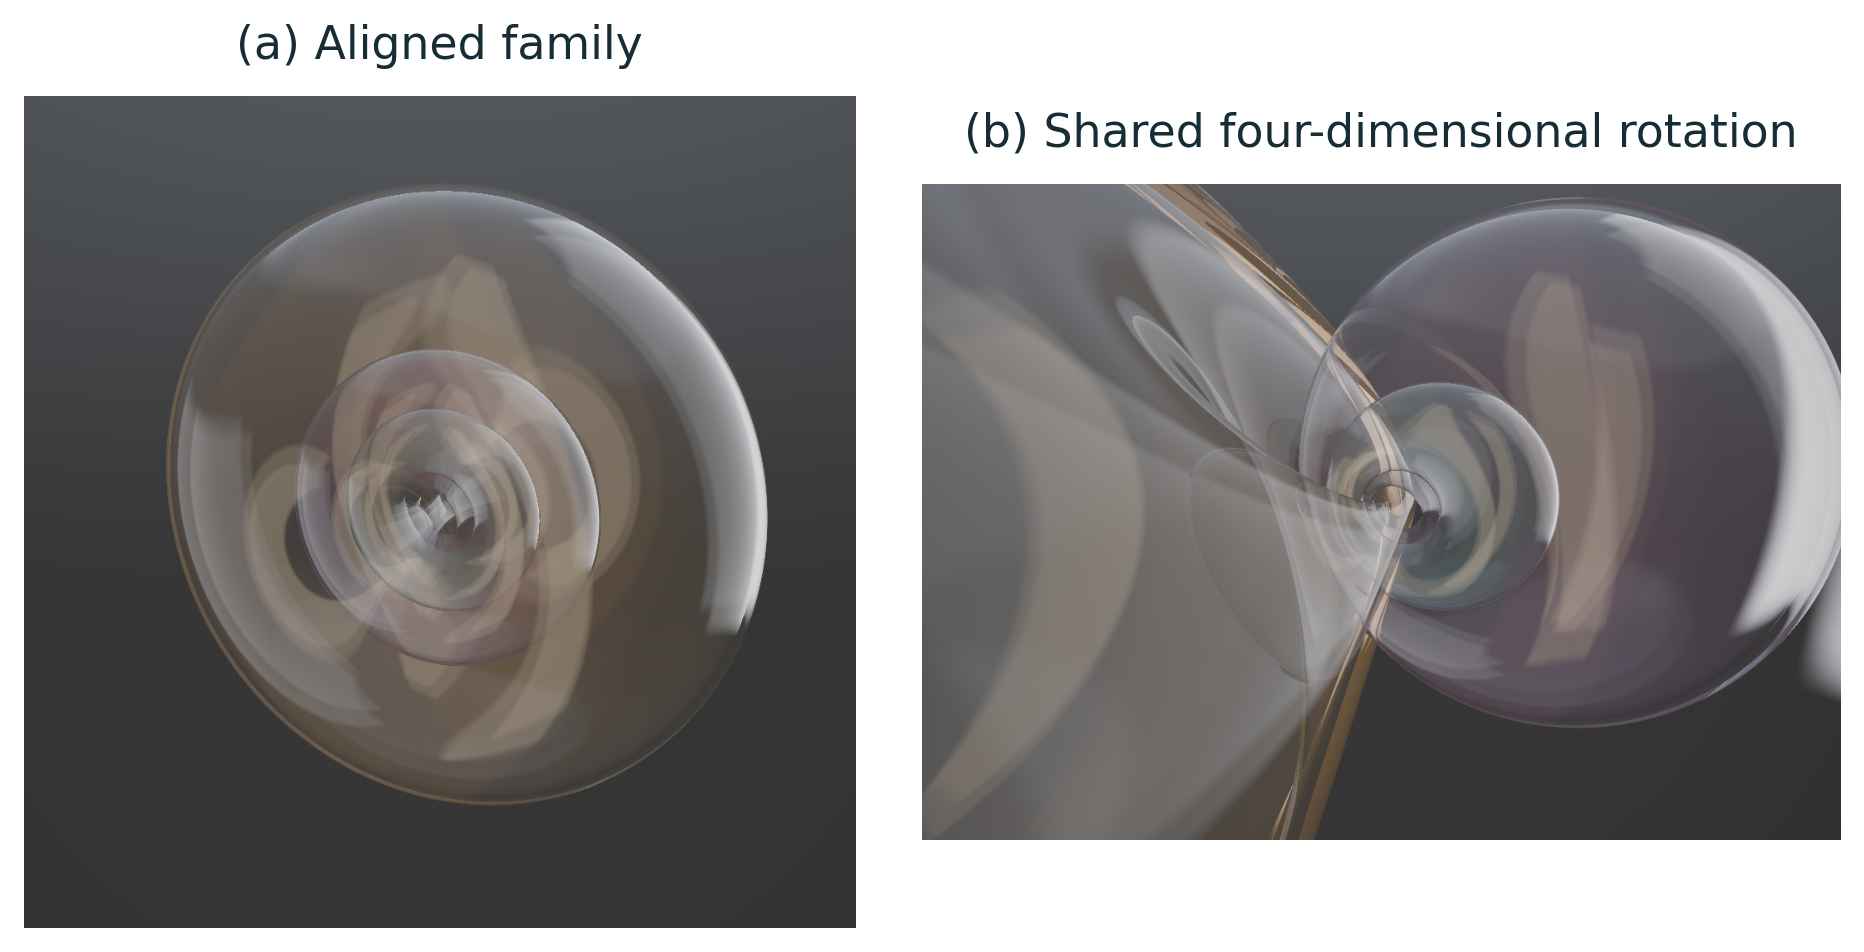
\includegraphics[width=1\linewidth,height=\textheight,keepaspectratio,alt={Three tori with parameters 25°, 45°, and 65°, rendered directly by the production shader. Each has a 0.5° shell, refractive index 1.3, and a small tinted coating. The second view applies a shared four-dimensional rotation. Camera and material values are recorded with the supplementary data.}]{figures/three-tori.png}
\caption{Three tori with parameters 25°, 45°, and 65°, rendered directly
by the production shader. Each has a 0.5° shell, refractive index 1.3,
and a small tinted coating. The second view applies a shared
four-dimensional rotation. Camera and material values are recorded with
the supplementary data.}\label{fig:family}
\end{figure}

\subsection*{Contributions}\label{contributions}
\addcontentsline{toc}{subsection}{Contributions}

This project contributes (i) a projector-based derivation of
stereographic ray intersections and normals, including why the problem
is intrinsically quartic; (ii) directly constructed Bernstein
coefficients in near/reciprocal charts, with closest-point recentering
and homogeneous-form polishing; (iii) multi-region solid and shell
optics, including \(0.01^\circ\) parameter bands; (iv) an evaluation
that separates input rounding, coefficient construction and root
solving; and (v) higher-precision construction in WebGL, with iterative
and closed-form solvers compared on it. Each ingredient has prior work.
The result is the first exact rendering of this family we know of:
published visualizations we have found use polygon meshes, tubes or
sampled distance fields.

\section{A family of tori and a coordinate on the
three-sphere}\label{a-family-of-tori-and-a-coordinate-on-the-three-sphere}

Write a point \(q=(q_1,q_2,q_3,q_4)^T\) of \(S^3\subset\mathbb R^4\) as
two complex coordinates \(z_1=q_1+iq_2\) and \(z_2=q_3+iq_4\), with
\(|z_1|^2+|z_2|^2=1\). For \(0<t<\pi/2\) define

\[
X(t,u,v)=(\cos t\cos u,\cos t\sin u,\sin t\cos v,\sin t\sin v)^T.
\]

For each fixed \(t\), the image \(T_t\) is
\(S^1(\cos t)\times S^1(\sin t)\). The angles \(u,v\) locate a point on
this torus; \(t\) selects the two circle radii. The identity
\(|X(t,u,v)|^2=\cos^2t+\sin^2t=1\) places every member in \(S^3\). At
\(t=\pi/4\) this is the standard Clifford torus, obtained by dividing
\((\cos u,\sin u,\cos v,\sin v)\) by \(\sqrt{2}\). Every point away from
the two circles \(z_1=0\) and \(z_2=0\) has a unique value

\[
\tau(q)=\operatorname{atan2}\!\left(\sqrt{q_3^2+q_4^2},\sqrt{q_1^2+q_2^2}\right).
\]

With \(u,v\) taken modulo \(2\pi\), \(X\) gives coordinates on the
complement of those circles: \((0,\pi/2)\times T^2\). Thus the family
foliates that complement by disjoint tori. At \(t=0\) the \(v\)-circle
collapses, and at \(t=\pi/2\) the \(u\)-circle collapses; including
these endpoint images gives all of \(S^3\). For \(q\in S^3\), membership
in \(T_t\) is exactly \(q_1^2+q_2^2=\cos^2t\). We use \(X\) for the
parameterization and \(q\) for a point on the sphere throughout.

For the Hopf map

\[
H(z_1,z_2)=\bigl(2\operatorname{Re}(z_1\overline{z_2}),\ 2\operatorname{Im}(z_1\overline{z_2}),\ |z_1|^2-|z_2|^2\bigr),
\]

\(H(T_t)\) is the latitude with third coordinate \(\cos 2t\). These are
therefore Hopf tori. An arbitrary rotation in \(SO(4)\) transports this
description to a correspondingly rotated Hopf fibration; it need not
preserve the particular fixed Hopf map written above.

Recovering \(t\) on \(S^3\) supplies a level-set membership test. To use
it for projected ray tracing, the remaining issue is the curve on
\(S^3\) corresponding to a straight ray in the projected scene.

\section{Lifting a 3D ray: a circle, not a straight 4D
ray}\label{lifting-a-3d-ray-a-circle-not-a-straight-4d-ray}

Use the north pole \(N=(0,0,0,1)\) and stereographic projection

\[
\sigma(q)=\frac{q_{1:3}}{1-q_4}.
\]

For \(p=(x,y,z)\), let \(D=1+|p|^2\) and

\[
V(p)=(2x,2y,2z,|p|^2-1),\qquad Q(p)=\frac{V(p)}D.
\]

Direct substitution gives \(|Q(p)|=1\) and \(\sigma(Q(p))=p\). Therefore
every point on the lifted ray \(Q(o+s d)\) is already on \(S^3\).
Intersecting a straight 4D ray with the hypersphere and then testing one
or two sphere hits would not solve the projected ray-tracing problem.

The lift of the complete 3D line, together with \(N\), is a circle. To
see this, choose independent vectors \(e_1,e_2\) perpendicular to its
direction \(d\). The line obeys \(e_i\cdot p=e_i\cdot o\), so its lift
obeys

\[
e_i\cdot q_{1:3}=(e_i\cdot o)(1-q_4),\qquad i=1,2.
\]

These are two affine hyperplanes in \(\mathbb R^4\), both containing
\(N\). Their common two-plane cuts the unit sphere in a circle. A
forward camera ray lifts to an arc ending at \(N\) as \(s\to+\infty\).

The desired intersections are precisely the points along this arc at
which the torus coordinate has the chosen value. The rational map \(Q\)
turns that test into the ray polynomial below.

\subsection{Why the intersection is a
quartic}\label{why-the-intersection-is-a-quartic}

The lifted line is a great circle only when its plane passes through the
origin of \(\mathbb R^4\), that is, when it also contains \(-N\). Since
\(\sigma(-N)=0\), this happens exactly for lines through the origin of
the projected space. On a great circle \(q=a\cos\varphi+b\sin\varphi\),
the membership condition \(q^TPq=c\) is a homogeneous quadratic in
\((\cos\varphi,\sin\varphi)\), so it is quadratic in \(\tan\varphi\).
Every other line lifts to a smaller circle
\(q=m+r(a\cos\varphi+b\sin\varphi)\) with \(m\neq0\). Then \(q^TPq\)
contains constant, first and second harmonics of \(\varphi\), and the
condition becomes a quartic in \(\tan(\varphi/2)\).

There is a planar picture of the same fact. \(P\) projects onto a
two-plane, and \(q^TPq=|Pq|^2\). Projecting the lifted circle into that
plane gives an ellipse, possibly degenerate, while the torus becomes the
circle of radius \(\cos t\) about the origin. The intersections are the
points where the ellipse crosses that circle, of which there are at most
four. The ellipse depends only on the ray and \(P\), so every torus in a
family sharing \(P\) is a different circle in the same picture.

The projected tori are Dupin cyclides, which are quartic surfaces
{[}1{]}; a line can meet one four times, so no method avoids a
degree-four problem for these images. A different projection could
straighten the lifted rays, but it would lose what makes the images
worth drawing. By Liouville's theorem the conformal maps from \(S^3\) to
\(\mathbb R^3\) are stereographic projections followed by Möbius
transformations. By Beltrami's theorem the maps that send great circles
to straight lines are central projections up to projective
transformation, and none of these is conformal. Gnomonic projection, for
example, turns the tori into quadrics with quadratic intersections, but
distorts their shape.

\begin{figure}[H]
\centering
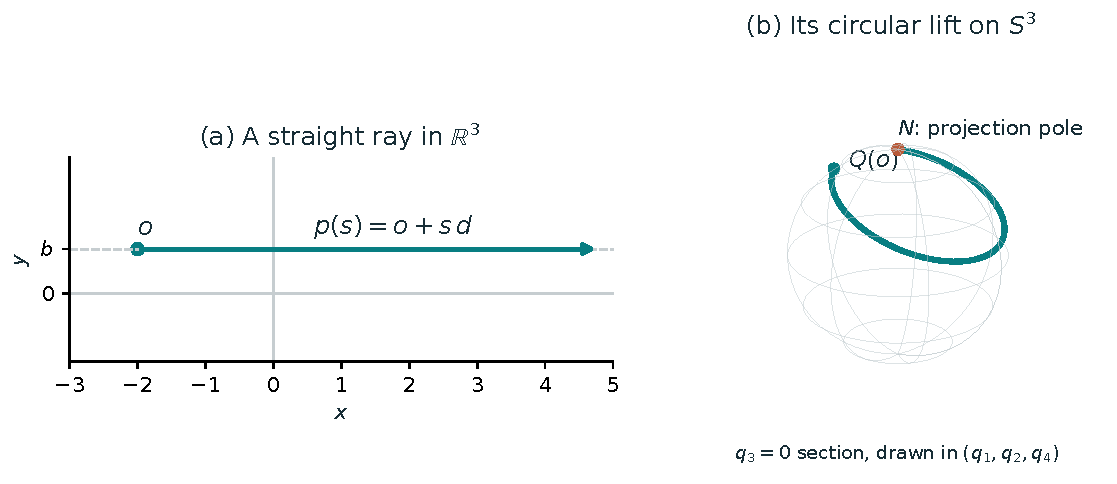
\includegraphics[width=1\linewidth,height=\textheight,keepaspectratio,alt={A straight ray and its circular lift. This diagram uses the section p=(s,b,0), so q\_3=0 and the relevant part of S\^{}3 can be drawn with coordinates (q\_1,q\_2,q\_4). The forward arc approaches the projection pole N. The diagram illustrates the mapping; it is not a surface-rendering approximation.}]{figures/ray-lift.pdf}
\caption{A straight ray and its circular lift. This diagram uses the
section \(p=(s,b,0)\), so \(q_3=0\) and the relevant part of \(S^3\) can
be drawn with coordinates \((q_1,q_2,q_4)\). The forward arc approaches
the projection pole N. The diagram illustrates the mapping; it is not a
surface-rendering approximation.}\label{fig:lift}
\end{figure}

\section{Rotation and the implicit
quartic}\label{rotation-and-the-implicit-quartic}

Let \(R\in SO(4)\) and

\[
P_0=\operatorname{diag}(1,1,0,0),\qquad P=RP_0R^T,\qquad c=\cos^2t.
\]

The rotated torus is parameterized by \(RX(t,u,v)\). Applying the
unrotated membership test to \(R^Tq\) characterizes it by \(q^TPq=c\) on
\(S^3\). The matrix \(P\) is a symmetric rank-two orthogonal projector:
\(P^T=P\), \(P^2=P\), and \(\operatorname{tr}P=2\).

The implementation constructs \(R\) by successively left-multiplying
rotations in the six coordinate planes. Changing their order generally
changes the result. Every supported rotation still uses the same
projector and intersection formulas.

The six rotation parameters do not give six independent geometric
degrees of freedom for the torus. For \(H=\operatorname{diag}(H_1,H_2)\)
with \(H_1,H_2\in SO(2)\),

\[
HP_0H^T=P_0,\qquad (RH)P_0(RH)^T=RP_0R^T.
\]

These two rotations shift the circle phases \(u,v\) without changing the
surface. The full stabilizer of \(P_0\) within \(SO(4)\) is
\(S(O(2)\times O(2))\), the block-diagonal orthogonal matrices with
total determinant one; its identity component is \(SO(2)\times SO(2)\).
Thus the projectors form the unoriented Grassmannian of two-planes in
\(\mathbb R^4\),

\[
\operatorname{Gr}_2(\mathbb R^4)\cong SO(4)/S(O(2)\times O(2)),\qquad
\dim\operatorname{Gr}_2(\mathbb R^4)=6-2=4.
\]

This is the standard projector/quotient description of the Grassmannian
{[}10{]}. At fixed \(t\), the torus therefore has four continuous
rotational degrees of freedom; allowing \(t\) to vary adds one. At
\(t=\pi/4\), \(P\) and \(I-P\) additionally describe the same boundary,
a discrete identification that leaves the dimension unchanged but
reverses the field sign used to select a solid's material side. The six
sliders provide a convenient redundant description of \(R\); the
redundancy need not correspond to two individual sliders in an ordered
product of fixed-plane rotations.

Substitute \(q=Q(p)\) and multiply by the strictly positive \(D^2\):

\[
\boxed{f_c(p)=V(p)^TPV(p)-c(1+|p|^2)^2=0.}
\]

Since \(V^TV=D^2\), it is convenient to put \(A_c=P-cI\) and write
\(f_c=V^TA_cV\). This is a polynomial of degree at most four; no
approximation has been introduced by clearing the denominator. In
computation the bounded field

\[
F_c(p)=Q(p)^TA_cQ(p)=\frac{f_c(p)}{D^2}
\]

has the same zero set and sign, while avoiding the quartic growth of
\(f_c\) far from the origin.

As a useful check, with \(R=I\) and \(\rho=\sqrt{x^2+y^2}\) the equation
is

\[
4\rho^2=c(1+\rho^2+z^2)^2.
\]

Taking the nonnegative square root and completing the square gives

\[
(\rho-\sec t)^2+z^2=\tan^2t.
\]

Thus the aligned projection is an ordinary ring torus with major radius
\(\sec t\) and minor radius \(\tan t\).

\section{Exact normals}\label{exact-normals}

Differentiate the quadratic form, using symmetry of \(P\),
\(\partial V/\partial p_i=2e_i+2p_i e_4\), and
\(\partial D/\partial p_i=2p_i\). The result is

\[
\boxed{\nabla f_c=4\left[(PV)_{1:3}+p\bigl((PV)_4-cD\bigr)\right].}
\]

Equivalently,

\[
\nabla f_c=4D\left[(A_cQ)_{1:3}+p(A_cQ)_4\right].
\]

The shader normalizes the expression in brackets. Its positive omitted
factor does not affect the normal direction. On the surface,
\(\nabla F_c=\nabla f_c/D^2\), so either field yields the same
orientation.

For \(0<c<1\), the level is regular on \(S^3\): the tangential gradient
of \(q^TPq\) is \(2(Pq-cq)\), whose squared norm on the level is
\(4c(1-c)>0\). Stereographic projection is a smooth coordinate map at
every finite point. The finite projected surface is consequently smooth
even when another part of it passes through infinity. A tangent ray is a
multiple polynomial root, not a singular point of the surface.

\section{The ray polynomial}\label{the-ray-polynomial}

For a unit direction \(d\), write \(p(s)=o+s d\) and

\[
v_0=(2o,|o|^2-1),\qquad v_1=(2d,2o\cdot d),\qquad v_2=(0,0,0,1).
\]

Then \(V(p(s))=v_0+s v_1+s^2v_2\). For the symmetric bilinear form
\(B(a,b)=a^TA_cb\),

\[
f_c(o+s d)=a_0+a_1s+a_2s^2+a_3s^3+a_4s^4,
\]

where

\[
\begin{aligned}
a_0&=B(v_0,v_0), & a_1&=2B(v_0,v_1),\\
a_2&=B(v_1,v_1)+2B(v_0,v_2), & a_3&=2B(v_1,v_2),\\
a_4&=B(v_2,v_2)=P_{44}-c.
\end{aligned}
\]

Positive real roots are forward intersections. A generic line has at
most four intersections with one boundary. Reflection or refraction
changes the direction, after which the same calculation is repeated for
the new ray. A shell uses two such quartics and can have eight crossings
along a single straight line.

\section{The projection pole and apparent
eversion}\label{the-projection-pole-and-apparent-eversion}

The pole lies on the rotated torus exactly when

\[
N^TPN=c\quad\Longleftrightarrow\quad P_{44}=c.
\]

This is also exactly the condition \(a_4=0\). The ray polynomial then
has degree at most three, with further reductions possible for special
rays. Finite roots remain legitimate intersections; a root at the
compactified endpoint representing infinity is not a finite hit.

The torus remains embedded and smooth in \(S^3\) throughout the
rotation. Its Euclidean projection becomes unbounded when the pole is on
the surface. Passing through that configuration can exchange the bounded
and unbounded sides of the selected material. The resulting inside-out
motion is not an eversion through a self-intersecting family of compact
tori in \(\mathbb R^3\): the family passes through infinity.

This visualization has clear antecedents. Banchoff describes the
stereographic images of rotated Clifford tori as Dupin cyclides,
explicitly including passage through infinity and interchange of
latitude and longitude. The UCI/3D-XplorMath gallery also displays this
inside-out deformation. These effects are prior work, not discoveries of
this implementation.
\href{https://www.math.brown.edu/tbanchof/Beyond3D.new/chapter6/s6_8.html}{Banchoff,
\emph{Beyond the Third Dimension}, online chapter};
\href{https://webapps.math.uci.edu/~vmm/Surface/clifford_torus/clifford_torus.html}{3D-XplorMath
Clifford torus gallery}.

\begin{figure}[H]
\centering
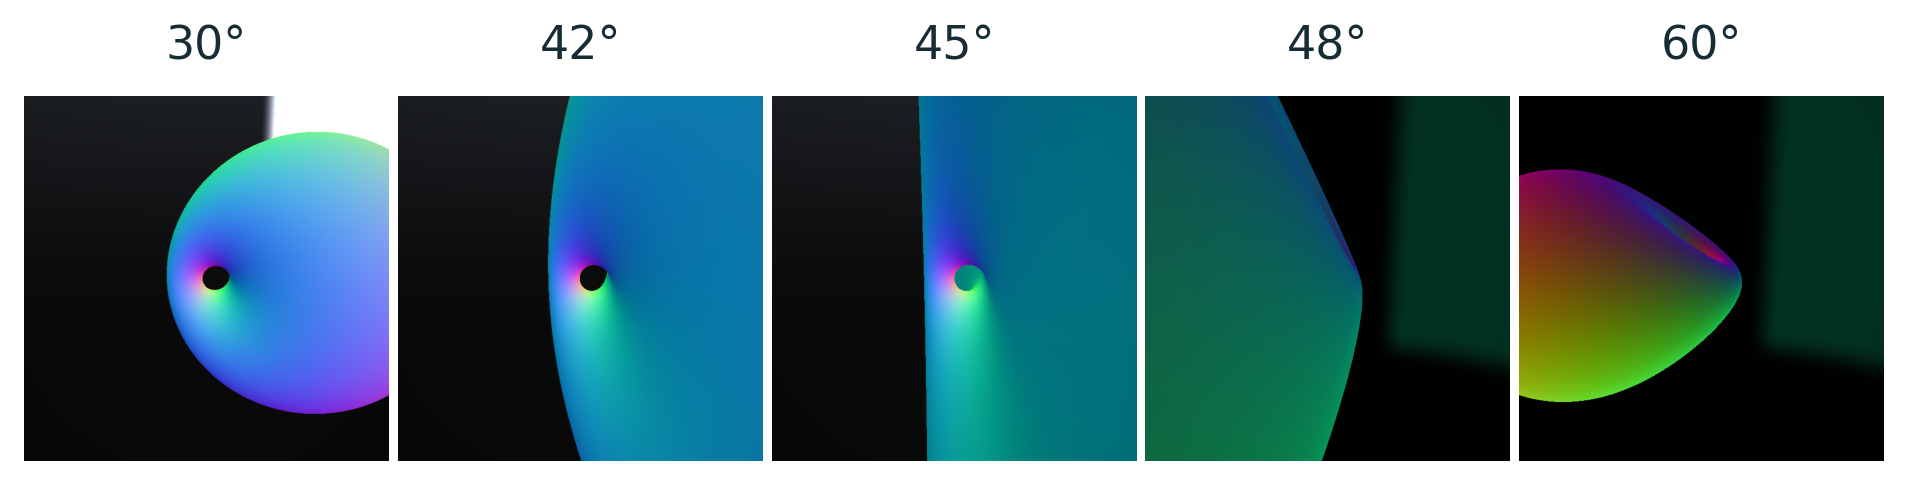
\includegraphics[width=1\linewidth,height=\textheight,keepaspectratio,alt={An XW rotation through the pole for the Clifford torus, at a fixed camera. The central panel has P\_\{44\}=\textbackslash cos\^{}2t in exact arithmetic. Colors encode the oriented analytic normal; the visible boundary leaves the image and returns with the material orientation carried through the rotation. These are ray-traced images, including at the unbounded configuration.}]{figures/pole-sequence.png}
\caption{An XW rotation through the pole for the Clifford torus, at a
fixed camera. The central panel has \(P_{44}=\cos^2t\) in exact
arithmetic. Colors encode the oriented analytic normal; the visible
boundary leaves the image and returns with the material orientation
carried through the rotation. These are ray-traced images, including at
the unbounded configuration.}\label{fig:pole}
\end{figure}

\section{Numerical intersection method used by the
demo}\label{numerical-intersection-method-used-by-the-demo}

\subsection{Recenter the line}\label{recenter-the-line}

Expanded camera-origin coefficients can be poorly conditioned when a
small torus feature is far along a ray. The implementation first sets

\[
k=o\cdot d,\qquad C=o-kd,\qquad p(s)=C+(k+s)d.
\]

Thus \(C\) is the closest point of the line to the origin. The line is
split into \(C+\lambda e\) with \(e=d\) or \(e=-d\) and
\(\lambda\geq0\). Candidates map back to \(s=\lambda-k\) or
\(s=-\lambda-k\) and are filtered and ordered in the original
forward-ray coordinate.

\subsection{Cover each half-line with two finite
charts}\label{cover-each-half-line-with-two-finite-charts}

Let \(L=\max(1,|C|)\). Use \(x=\lambda/L\) on \(0\leq\lambda\leq L\),
and \(x=L/\lambda\) on \(L\leq\lambda<\infty\). Both coordinates lie in
\([0,1]\), but \(x=0\) in the reciprocal chart denotes infinity and is
excluded. No finite far clipping sphere is introduced. The coordinate
\(x=1\) is the common chart boundary; repeated intersection queries
apply the ordinary positive-distance cutoff there.

Define

\[
a=(2C/L^2,(|C|^2-1)/L^2),\quad
b=(2e/L,2C\cdot e/L),\quad c_2=(0,0,0,e\cdot e).
\]

The near numerator is \(W(x)=a+bx+c_2x^2=V(C+Lxe)/L^2\). The reciprocal
numerator reverses the coefficients:
\(W(x)=c_2+bx+ax^2=x^2V(C+Le/x)/L^2\). Thus \(g(x)=W(x)^TA_cW(x)\) has
exactly the finite intersections of its chart. The common scale
\(L^{-2}\) limits coefficient growth. Although \(C\cdot e=0\) and
\(e\cdot e=1\) in exact arithmetic, the code retains their computed
values.

For either chart write \(W=a'+b'x+c'x^2\) and set \(w_0=a'\),
\(w_1=a'+b'/2\), \(w_2=a'+b'+c'\). Its quartic Bernstein coefficients
are

\[
\begin{aligned}
b_0&=B(w_0,w_0), & b_1&=B(w_0,w_1),\\
b_2&=\bigl(B(w_0,w_2)+2B(w_1,w_1)\bigr)/3,\\
b_3&=B(w_1,w_2), & b_4&=B(w_2,w_2).
\end{aligned}
\]

A strictly one-signed coefficient set rejects the chart by the Bernstein
convex-hull property. Degree reduction needs no division by a small
leading monomial coefficient. In the reciprocal chart, a relative
perturbation of \(x\) gives approximately the same relative perturbation
of \(\lambda=L/x\); distant intersections therefore retain relative
coordinate resolution as they approach \(x=0\).

\subsection{Isolate and polish roots}\label{isolate-and-polish-roots}

A real polynomial is monotone between consecutive roots of its
derivative. The solver obtains the derivative roots recursively,
starting with a linear equation, then partitions the quadratic, cubic
and quartic into monotone intervals. Coefficient differences supply
Bernstein derivatives; omitted positive degree factors do not affect
their zeros. De Casteljau evaluation is used throughout.

Opposite signs at interval ends bracket a crossing. Up to 25 bisection
steps are followed by secant interpolation inside the final bracket,
preserving relative accuracy for roots near zero. Near-zero stationary
values supply even-multiplicity candidates only when adjacent intervals
do not already contain crossings. Endpoints require exact zero.
Coefficients are rescaled, and duplicate candidates are compared
relative to their chart coordinates.

Up to four bounded Newton steps polish each candidate against the
homogeneous form itself:

\[
g=W^TA_cW,\qquad g'=2(b'+2xc')^TA_cW.
\]

A proposal is accepted only if it stays in \([0,1]\), moves by at most
\(0.05\max(x,10^{-6})\), and strictly decreases the computed \(|g|\).
Refinement stops at a computed zero, zero derivative, float stagnation
or rejected proposal; nonfinite residuals cannot pass the decrease test.
This guard retains the previous candidate when progress is unresolved.
It does not preserve the isolator's final bracket, and a decrease in a
rounded residual does not certify a smaller geometric distance error.
Define \(M=|W|^T|A_c||W|\), where absolute values are componentwise. The
acceptance residual is

\[
\rho=\frac{|g|}{M+|g'|h},\qquad
h=\begin{cases}1&\text{near chart},\\x&\text{reciprocal chart}.\end{cases}
\]

The shader requires \(\rho<2\times10^{-6}\), a finite converted
distance, and a forward hit beyond the self-intersection cutoff. The
reciprocal factor \(x\) scales the derivative term to relative distance
error. This is a conditioning-aware heuristic, not a certified
distance-error bound. Charts are visited in ray order: negative
reciprocal, negative near, positive near, positive reciprocal, omitting
the negative half when it lies behind the origin.

\subsection{Limits of the float32
method}\label{limits-of-the-float32-method}

The stationary-point tolerance called \texttt{errorBound} in the shader
is a heuristic, not an interval bound. Close roots can merge,
near-tangent contacts can appear or vanish, and very distant roots are
limited by float32 range and resolution. Near the pole, rounding the
rotation or level to float32 can move a remote root a long way. Section
11 measures these effects and shows where they originate. A line
contained in the surface gives an identically zero polynomial; it has no
isolated first crossing and is not rendered as one.

Let \(\gamma\) be the smallest distinct angular boundary separation
among enabled tori. The bias scale is
\(\beta=\operatorname{clamp}(0.05\gamma,10^{-6},4\times10^{-4})\), with
\(\gamma\) in radians; a lone solid uses the upper limit. The
ray-distance cutoff is \(\beta\max(1,|o|)/2\) and the post-hit offset is
\(\beta\max(1,|p|)\). These suppress self-intersections while retaining
the tested \(0.01^\circ\) walls. Features below the offset and float32
resolution remain unresolved. ``No finite clipping sphere'' therefore
does not mean unlimited numerical reach or guaranteed detection of every
mathematical root.

\section{A solid and a shell are different material
choices}\label{a-solid-and-a-shell-are-different-material-choices}

An implicit equation specifies a boundary. Refraction also requires a
choice of which side contains which medium.

\subsection{Solid mode: one torus
boundary}\label{solid-mode-one-torus-boundary}

Solid mode chooses glass where \(F_c>0\), equivalently \(q^TPq>c\). In
the unrotated case this is the familiar filled tube bounded by the ring
torus. In \(S^3\) it is the side \(\tau<t\), whose closure is a solid
torus. Its outward normal is

\[
n_{\mathrm{out}}=-\frac{\nabla f_c}{|\nabla f_c|}.
\]

A single closed torus boundary is sufficient to define this solid. A ray
can enter the tube and later exit through another point on the same
boundary. A second torus is not needed to obtain entry and exit
intersections.

When \(P_{44}>c\), the pole is inside the chosen material region, so its
projection includes the exterior of a sufficiently large ball. The
definition of the material is held fixed during animation; the program
does not silently swap glass and air to keep glass bounded.

\subsection{Shell mode: two neighboring
tori}\label{shell-mode-two-neighboring-tori}

Set \(t_-=t-\Delta t/2\) and \(t_+=t+\Delta t/2\), with both in
\((0,\pi/2)\), and define

\[
c_{\mathrm{low}}=\cos^2t_+,\qquad c_{\mathrm{high}}=\cos^2t_-.
\]

Because cosine squared decreases on this interval,
\(c_{\mathrm{low}}<c_{\mathrm{high}}\). Glass now occupies

\[
\boxed{c_{\mathrm{low}}<Q(p)^TPQ(p)<c_{\mathrm{high}}.}
\]

Equivalently, glass is \(t_-<\tau(R^TQ(p))<t_+\). Both adjoining regions
are air. The shell is bounded by the two independently solved quartics
\(f_{c_{\mathrm{low}}}=0\) and \(f_{c_{\mathrm{high}}}=0\). Each tracing
step selects the nearest positive hit from either equation. At the low
boundary the outward normal is the \textbf{negative} gradient; at the
high boundary it is the \textbf{positive} gradient. Those opposite signs
make cavity entry and exit obey the same optical code as outer-wall
entry and exit.

This is an exact parameter-band shell, not a constant-thickness
Euclidean offset surface. In \(S^3\), the \(t\) direction is normal to
the tori and \(|\partial X/\partial t|=1\), so \(\Delta t\) has a
natural angular thickness interpretation. Stereographic projection has
metric factor \(2/(1+|p|^2)\): a sufficiently thin shell has local
Euclidean normal thickness approximately \((1+|p|^2)\Delta t/2\), with
\(\Delta t\) in radians. Near infinity that local approximation is not
uniform.

The UI defaults to the minimum width of \(0.01^\circ\), and caps width
at \(30^\circ\) or the smaller amount needed to keep both endpoints
between \(0.25^\circ\) and \(89.75^\circ\). A boundary reaches infinity
when \(P_{44}\) equals its level. Glass itself extends to infinity when
\(P_{44}\) lies strictly between the two levels; in that case both
boundary surfaces can be bounded while the region between them through
infinity is unbounded.

\begin{figure}[H]
\centering
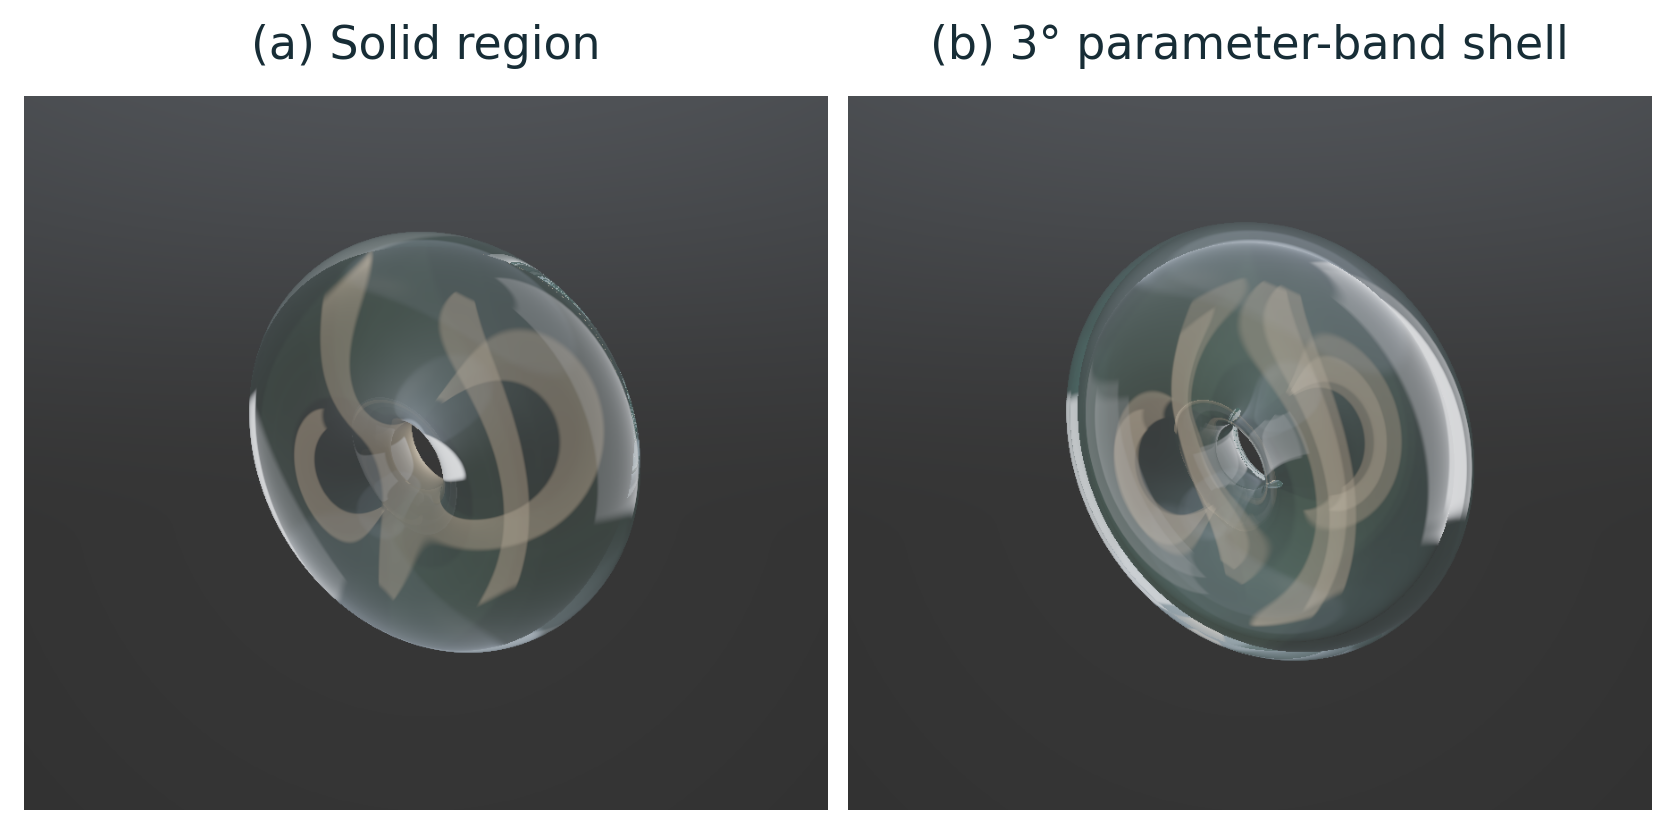
\includegraphics[width=0.9\linewidth,height=\textheight,keepaspectratio,alt={A single solid torus and a shell between two nearby tori, with the same camera, central parameter t = 45°, refractive index 1.45, environment, and coating setting. The shell width here is 3° to make the two-wall structure visible. Entry and exit use genuine intersections with the respective material boundaries.}]{figures/solid-shell.png}
\caption{A single solid torus and a shell between two nearby tori, with
the same camera, central parameter t = 45°, refractive index 1.45,
environment, and coating setting. The shell width here is 3° to make the
two-wall structure visible. Entry and exit use genuine intersections
with the respective material boundaries.}\label{fig:materials}
\end{figure}

\subsection{Several material regions}\label{several-material-regions}

Up to three tori share the same \(P\) but have independent parameter
intervals and optical properties. At each step, the nearest boundary
among the enabled regions is selected. When regions overlap, the
narrower interval in \(Q^TPQ\) takes precedence; the higher-numbered
slot breaks ties. Coincident level boundaries update membership
together. This explicit convention preserves nested media as their
projections change orientation; it is an application choice, not a
geometric necessity. Chrome follows the same material region through the
pole and may become the exterior medium.

\section{All the optics occur in ordinary
3D}\label{all-the-optics-occur-in-ordinary-3d}

The four-dimensional geometry defines the surface and material
membership. Camera rays, distances, illumination, normals, reflection,
absorption, and refraction are evaluated in Euclidean \(\mathbb R^3\).
Stereographic projection preserves angles, but the implementation does
not transport a physical 4D optical simulation into 3D.

For unit incident direction \(d\), orient the surface normal \(n\)
against the ray and let \(c_i=-n\cdot d\). With refractive indices
\(n_1\) and \(n_2\) on the incident and transmitted sides, put
\(\eta=n_1/n_2\). Then

\[
r=d+2c_i n,\qquad K=1-\eta^2(1-c_i^2).
\]

If \(K<0\), total internal reflection occurs. Otherwise the transmitted
direction is

\[
d_{\mathrm{tr}}=\eta d+(\eta c_i-\sqrt K)n.
\]

This is Snell's law in vector form. The shader uses the unpolarized
dielectric Fresnel reflectance, averaging the squared s- and
p-polarization amplitudes, and follows the resulting reflected and
transmitted directions. Medium membership is initialized from the ray
origin. A crossing updates it using the outward normal; a grazing
contact is treated as a silhouette contact without toggling the medium.
Numerical grazing thresholds remain approximations.

The procedural angular environment has a grid, checker pattern, bright
strips, and colored lights that make bending visible. It is a
direction-dependent distant environment, not a finite checkerboard
floor. Opacity blends a locally lit colored coating at each interface
and also scales Beer-style absorption in glass. It is consequently not a
pure bulk extinction coefficient or a physically complete material
parameterization.

The main path allows 8, 16, or 24 interactions according to quality. At
the first interface, the reflected branch can intersect the object for
up to four further interfaces; later reflection contributions use the
environment directly. Total internal reflection continues within the
same medium. Remaining energy after the transport budget is resolved to
the environment. Segment absorption is capped, and rays remaining in an
unbounded material use finite absorption. There is no complete recursive
ray tree, spectral dispersion, global illumination, or caustic
calculation. Exact surface equations and Snell-law directions should not
be confused with exact light transport.

\section{Validation of the float32
renderer}\label{validation-of-the-float32-renderer}

\subsection{Regression checks and thin-shell
optics}\label{regression-checks-and-thin-shell-optics}

All 24 JavaScript CPU tests pass. They check projector invariants,
polynomial identities, finite-difference normals, analytic ring-torus
roots, tangencies, degree reduction, material membership and thin-wall
origin offsets. Five independent-reference tests, including an exact
rational double tangent, and five analysis tests of the matching code
also pass. On an Apple M3 Pro, the native offscreen GPU suite passes 625
solid, 403 shell and 133 three-torus ray cases, plus 31 focused
thin-shell sequences.

Instrumented transport checks hit positions, successive media,
refractive indices, analytic normals, Snell directions and total
internal reflection. All 36 paths pass, covering 392 events. At
\(\Delta t=0.01^\circ\), aligned single shells at
\(t=1^\circ,5^\circ,25^\circ,45^\circ,65^\circ,85^\circ,89^\circ\) each
retain eight crossings, and three shells retain all 24, with twelve
entries and twelve exits. The paths include oblique rays and both
pole-crossing boundaries. The largest Snell residual is
\(1.05\times10^{-7}\) and the largest normal error
\(9.74\times10^{-8}\). Thirty-one index-one, opacity-zero checks show no
colour change. Event counts and source hashes are in
\texttt{docs/gpu-results.json}.

\subsection{Independent reference and
protocol}\label{independent-reference-and-protocol}

The reference expands \(V(o+sd)^T(P-cI)V(o+sd)\) in exact rational
arithmetic and isolates its real roots with SymPy 1.14's
continued-fraction method {[}9{]}, to brackets no wider than
\(10^{-30}\), keeping multiplicities. It shares no code with the
renderer. It is evaluated twice: on the exact binary values of the
float32 uniforms supplied to the GPU, which measures the solver, and on
the intended geometry at 80 significant digits, which measures input
rounding.

The designed corpus has 867 rays. Its 600 pole rays cover
\(t=25^\circ,45^\circ,65^\circ\) with an XW pole crossing and
\(t=45^\circ\) with an extra spatial rotation, each offset from the pole
by \(\delta=0\) and \(\delta=\pm10^{-k}\) for \(k=1,\ldots,12\). A
further 168 rays use both adjacent float32 values of \(P_{44}\) around
\(c\) for seven values of \(t\); others cover silhouettes, chart
junctions, the origin, a contained line and twelve seeded six-plane
rotations. The inputs and both reference root sets are in
\texttt{research/results/reference.json}.

Two baselines solve the same rays. The first adapts Peters's CC0 GLSL
implementation {[}11{]} of Yuksel's derivative-partitioned
Newton--bisection method {[}5{]}, in centered affine coordinates with a
Cauchy bound and in the same near/reciprocal charts. The second adapts
Schwarze's float32 Ferrari/Cardano solver {[}8{]}. Provenance and every
adaptation are recorded in \texttt{research/THIRD\_PARTY.md}.

Every method enumerates all distinct positive roots of the
\textbf{unchanged original ray}, with no origin advance, rendering bias
or far cutoff. Only identical float outputs are merged. Outputs are
matched one-to-one to reference roots, maximizing the number of matches
with
\(|s_{\mathrm{GPU}}-s_{\mathrm{ref}}|/\max(1,s_{\mathrm{ref}})\leq10^{-4}\).
A ray fails if any reference root or output is unmatched, or if any
output is not finite. Results are recorded before and after the shared
homogeneous refinement and residual filter.

\subsection{Designed corpus}\label{designed-corpus}

Native offscreen OpenGL, all 867 rays and 1,470 roots:

{
\Needspace{10\baselineskip}\begin{longtable}[]{@{}llrrr@{}}
\toprule\noalign{}
Method & Stage & Failed rays & Matched roots & Unmatched outputs \\
\midrule\noalign{}
\endhead
\bottomrule\noalign{}
\endlastfoot
Bernstein near/reciprocal & Raw & 0 & 1,470 & 0 \\
Bernstein near/reciprocal & Refined & 0 & 1,470 & 0 \\
Yuksel--Peters, centered & Raw & 0 & 1,470 & 0 \\
Yuksel--Peters, centered & Refined & 0 & 1,470 & 0 \\
Yuksel--Peters, near/reciprocal & Raw & 0 & 1,470 & 0 \\
Yuksel--Peters, near/reciprocal & Refined & 0 & 1,470 & 0 \\
Ferrari, centered & Raw & 428 & 682 & 223 \\
Ferrari, centered & Refined & 378 & 740 & 13 \\
\end{longtable}
}

\begin{figure}[H]
\centering
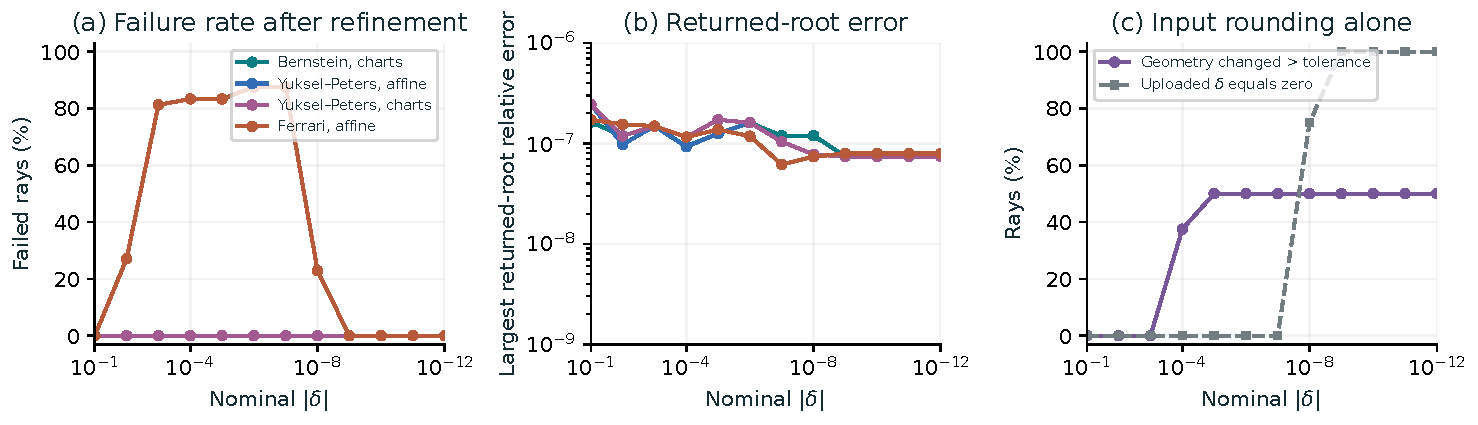
\includegraphics[width=1\linewidth,height=\textheight,keepaspectratio,alt={All-roots comparison versus nominal distance from the projection pole; each nonzero magnitude contains 48 rays. Left: failed-ray percentage after common refinement, with the three iterative variants overlapping at zero. Middle: largest returned-root relative error after refinement; missing roots must be read with the left panel. Right: disagreement caused by input rounding alone, and the proportion of uploaded inputs whose \textbackslash delta is exactly zero.}]{figures/pole-errors.pdf}
\caption{All-roots comparison versus nominal distance from the
projection pole; each nonzero magnitude contains 48 rays. Left:
failed-ray percentage after common refinement, with the three iterative
variants overlapping at zero. Middle: largest returned-root relative
error after refinement; missing roots must be read with the left panel.
Right: disagreement caused by input rounding alone, and the proportion
of uploaded inputs whose \(\delta\) is exactly zero.}\label{fig:errors}
\end{figure}

The three iterative variants match every root, with largest relative
error \(7.56\times10^{-5}\), from grazing rays; in the pole sweep the
largest error is \(1.63\times10^{-7}\) for Bernstein and
\(2.45\times10^{-7}\) for both Yuksel variants. The farthest
intersection is about \(2.40\times10^9\) scene units away. The float32
Ferrari port's 378 refined failures comprise 227 pole rays, 13 grazing
rays and 138 precision cases. On this corpus, the chart coordinates give
no completeness advantage over the centered baseline. Running the
production intersection function in WebGL 2 through ANGLE Metal, with
its normal origin advance, also passes all 867 rays
(\texttt{research/results/webgl-validation.json}).

Input rounding is a separate effect. At nominal \(|\delta|\leq10^{-9}\),
every pole-sweep input rounds to exactly \(P_{44}=c\), and the remote
root of the intended geometry disappears from the uploaded polynomial;
no solver can restore it. Across the pole corpus, rounding alone changes
the root set beyond tolerance on 210 of 600 rays.

\subsection{Seeded stress corpus}\label{seeded-stress-corpus}

A frozen revision was then evaluated on 2,400 seeded queries: 600
random, 600 pole, 600 exact or near-tangent, and 600 thin-shell
boundaries in 100 groups of three \(0.01^\circ\) shells. The tangent
family has 200 exact rational double contacts and two nearby rays per
contact. No solver was changed during this pass.

All 1,800 random, pole and shell queries pass, and every shell group
keeps its boundary order. All three iterative variants fail the same 109
grazing queries: 40 with too few outputs, 34 with too many and 35 with
misplaced ones. Bernstein matches 3,166 of 3,314 represented roots, and
each Yuksel variant 3,165. At tolerances \(10^{-5}\) and \(10^{-6}\) the
failure counts rise to 197/195/195 and 294/292/292 (Bernstein, centered
Yuksel, chart Yuksel). In WebGL the production renderer fails 123
grazing queries. Input rounding separately changes 570 intended root
sets.

Twelve predetermined optical paths through the shell groups pass
independent captured-ray checks of intersections, normals, media and
Snell directions for each solver: 167 boundaries, of which 158 are
optical events and nine are hidden boundaries. One path reaches the
boundary cap and one the energy cutoff. Thirty full-image comparisons
against Bernstein have largest frame-mean RGB error
\(2.82\times10^{-6}\); a single pixel differs by 0.341.
\texttt{research/STRESS.md} gives the constructions, failures and
commands.

\subsection{Refinement ablation}\label{refinement-ablation}

Four refinement policies were compared on the same Bernstein candidates
and acceptance filter. All four match every designed-corpus root; their
largest relative errors differ by subset:

{
\Needspace{10\baselineskip}\begin{longtable}[]{@{}
  >{\raggedright\arraybackslash}p{(\linewidth - 6\tabcolsep) * \real{0.2000}}
  >{\raggedleft\arraybackslash}p{(\linewidth - 6\tabcolsep) * \real{0.2667}}
  >{\raggedleft\arraybackslash}p{(\linewidth - 6\tabcolsep) * \real{0.2667}}
  >{\raggedleft\arraybackslash}p{(\linewidth - 6\tabcolsep) * \real{0.2667}}@{}}
\toprule\noalign{}
\begin{minipage}[b]{\linewidth}\raggedright
Refinement policy
\end{minipage} & \begin{minipage}[b]{\linewidth}\raggedleft
Pole sweep
\end{minipage} & \begin{minipage}[b]{\linewidth}\raggedleft
Precision cases
\end{minipage} & \begin{minipage}[b]{\linewidth}\raggedleft
Six-plane rotations
\end{minipage} \\
\midrule\noalign{}
\endhead
\bottomrule\noalign{}
\endlastfoot
None & \(2.37\times10^{-7}\) & \(2.35\times10^{-6}\) &
\(8.69\times10^{-7}\) \\
Step-limited, no decrease test & \(1.63\times10^{-7}\) &
\(1.75\times10^{-7}\) & \(1.23\times10^{-5}\) \\
Residual-decreasing (production) & \(1.63\times10^{-7}\) &
\(1.58\times10^{-7}\) & \(5.84\times10^{-6}\) \\
Noise-aware & \(2.37\times10^{-7}\) & \(2.35\times10^{-6}\) &
\(8.69\times10^{-7}\) \\
\end{longtable}
}

The noise-aware guard requires
\(|g_{\mathrm{new}}|+8\epsilon M_{\mathrm{new}}<|g|-8\epsilon M\) with
\(\epsilon=2^{-23}\), and in practice never moves a root. The production
guard keeps Newton's gains on the pole and precision subsets and halves
its worst rotation error, though that remains larger than with no
correction. Polishing in float32 helps on average but not uniformly.

\subsection{Rendering cost}\label{rendering-cost}

The full-render comparison replaces only the intersection and refinement
functions in the production shader, so timings include coefficient
construction, rejection, root finding and the resulting optical paths.
Native draw-plus-\texttt{glFinish} medians at 1280×720 with a
24-interaction cap, from three alternating blocks of ten frames:

{
\Needspace{10\baselineskip}\begin{longtable}[]{@{}lrrr@{}}
\toprule\noalign{}
Scene & Bernstein (production) & Yuksel, centered & Yuksel, charts \\
\midrule\noalign{}
\endhead
\bottomrule\noalign{}
\endlastfoot
One solid torus & 3.13 ms & 2.86 ms & 2.88 ms \\
One 0.01° shell & 5.63 ms & 6.38 ms & 5.55 ms \\
Three 0.01° shells, aligned & 19.78 ms & 33.02 ms & 22.27 ms \\
Three 0.01° shells, XW = 45° & 38.45 ms & 67.69 ms & 45.74 ms \\
\end{longtable}
}

Yuksel is slightly faster for one solid, the chart variant matches
Bernstein for one shell, and Bernstein is fastest for three shells, the
application's main workload. Both Yuksel renderers pass the full
transport suite. Raw samples, block medians and interquartile ranges are
in \texttt{research/results/renderer-benchmark.json}.

In Chrome 157 with WebGL 2 on ANGLE Metal, draw plus a synchronous
one-pixel readback takes the following medians of 30 frames:

{
\begin{minipage}{\linewidth}\centering\begin{tabular}{@{}lrr@{}}
\toprule\noalign{}
Scene, 24-interaction cap & 640 × 360 & 1280 × 720 \\
\midrule\noalign{}



One solid torus & 3.30 ms & 5.30 ms \\
Three 0.01° shells, aligned & 12.40 ms & 36.40 ms \\
Three 0.01° shells, XW = 45° & 25.00 ms & 91.90 ms \\
\bottomrule\end{tabular}\end{minipage}
}

\begin{figure}[H]
\centering
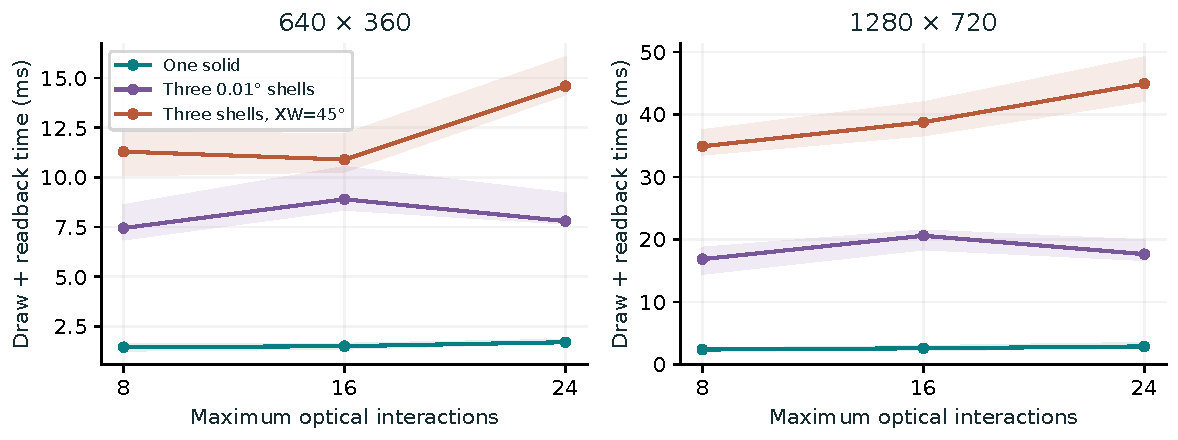
\includegraphics[width=1\linewidth,height=\textheight,keepaspectratio,alt={Browser draw-and-readback timings on Apple M3 Pro. Lines show medians; shading shows the interquartile range of 30 samples. The interaction count is a maximum budget, not a claim that every pixel encounters that many interfaces.}]{figures/performance.pdf}
\caption{Browser draw-and-readback timings on Apple M3 Pro. Lines show
medians; shading shows the interquartile range of 30 samples. The
interaction count is a maximum budget, not a claim that every pixel
encounters that many interfaces.}\label{fig:performance}
\end{figure}

\section{Where the grazing failures arise, and how to remove
them}\label{where-the-grazing-failures-arise-and-how-to-remove-them}

\subsection{Stage diagnosis}\label{stage-diagnosis}

GPU probes captured every intermediate quantity for the 600 grazing
queries: the centered ray, the chart vectors \(W\), the matrix \(P-cI\),
the polynomial coefficients, and the candidates before and after
refinement. Exact arithmetic then solved each captured stage, and each
was compared with the reference for the uploaded inputs. Every solver
gives the same counts:

{
\begin{minipage}{\linewidth}\centering\begin{tabular}{@{}lrr@{}}
\toprule\noalign{}
Stage solved or observed & Failed / 600 & Of final 109 \\
\midrule\noalign{}



Exact ray from captured \(C\) and \(k\) & 39 & 34 \\
Captured \(W\), exact \(P-cI\) & 103 & 88 \\
Captured \(W\), float32 \(P-cI\) & 106 & 90 \\
Exact roots of captured coefficients & 109 & 109 \\
GPU isolated candidates & 109 & 109 \\
Refined candidates, before filtering & 109 & 109 \\
Final accepted GPU roots & 109 & 109 \\
\bottomrule\end{tabular}\end{minipage}
}

Exact roots of the captured coefficients already fail on all 109
queries, with the same 40/34/35 breakdown. The intersections are lost or
moved while the polynomial is being built; isolation, refinement and
filtering neither cause nor repair the failures. Earlier rows are not
nested sets, because rounding errors partly cancel, so differences
between rows are not an error budget. Disabling Bernstein's proximity
merging changes no output, and the residual filter rejects no grazing
candidate. The
\href{https://github.com/tommyhax/hopf-observatory/blob/main/research/diagnostics/grazing/results/grazing-diagnostic.png}{stage-by-stage
traces} of three representative failures show pairs appearing, vanishing
and shifting during construction.

\subsection{Binary64 construction on the
CPU}\label{binary64-construction-on-the-cpu}

A CPU replay uses the project's JavaScript Bernstein solver in binary64,
on the same uploaded float32 geometry, with no polishing or residual
filter. It is fed either the float32 coefficients captured from the GPU
or coefficients rebuilt in binary64:

{
\Needspace{10\baselineskip}\begin{longtable}[]{@{}
  >{\raggedright\arraybackslash}p{(\linewidth - 8\tabcolsep) * \real{0.5128}}
  >{\raggedleft\arraybackslash}p{(\linewidth - 8\tabcolsep) * \real{0.1410}}
  >{\raggedleft\arraybackslash}p{(\linewidth - 8\tabcolsep) * \real{0.1410}}
  >{\raggedleft\arraybackslash}p{(\linewidth - 8\tabcolsep) * \real{0.1026}}
  >{\raggedleft\arraybackslash}p{(\linewidth - 8\tabcolsep) * \real{0.1026}}@{}}
\toprule\noalign{}
\begin{minipage}[b]{\linewidth}\raggedright
Construction and solving
\end{minipage} & \begin{minipage}[b]{\linewidth}\raggedleft
Failed / 600
\end{minipage} & \begin{minipage}[b]{\linewidth}\raggedleft
Matched / 584
\end{minipage} & \begin{minipage}[b]{\linewidth}\raggedleft
Missing
\end{minipage} & \begin{minipage}[b]{\linewidth}\raggedleft
Extra
\end{minipage} \\
\midrule\noalign{}
\endhead
\bottomrule\noalign{}
\endlastfoot
Native float32 GPU, refined & 109 & 436 & 148 & 137 \\
Float32 coefficients, binary64 solving & 109 & 434 & 150 & 138 \\
Binary64 construction and solving & \textbf{0} & \textbf{584} &
\textbf{0} & \textbf{0} \\
\end{longtable}
}

Solving the float32 coefficients more accurately changes nothing.
Rebuilding them in binary64 recovers every intersection, with largest
relative error \(4.87\times10^{-12}\); all queries still pass at
\(10^{-10}\), and 15 fail on position at \(10^{-12}\). Details are in
\texttt{research/diagnostics/double-precision/}.

\subsection{Paired float32 construction in
WebGL}\label{paired-float32-construction-in-webgl}

WebGL 2 has no double type, and Apple GPUs have no binary64 hardware in
any API. The browser variant therefore carries sensitive values as
unevaluated sums of two float32 values {[}14{]}. Sums use error-free
transformations, and products split each operand into two 12-bit halves
so that partial products are exact. GPU compilers may legally
reassociate float arithmetic, which would cancel the recovered error
terms. Each intermediate is therefore passed through an integer XOR with
a uniform that is always zero, so the compiler cannot see through it.
Eight arithmetic fixtures on the actual GPU check cancellation, product
residuals, division and widely separated scales before any root test
runs.

Paired arithmetic covers ray recentering, the chart vectors, \(P-cI\),
Bernstein coefficient construction, homogeneous residuals, derivatives
and the conversion back to ray distance. The coefficients are rounded to
float32 for the existing isolator, which may now take up to 48 bisection
steps; candidates are refined and accepted against the paired
homogeneous form. On both corpora this variant matches all 4,784
intersections, against 123 production failures, with largest relative
error \(2.16\times10^{-7}\). It passes the complete optical suite. An
intermediate version with 25 bisections failed one shell case, two
genuine intersections \(2.2\times10^{-9}\) apart near distance 5.009,
which exposed the insufficient isolation; the evidence is kept in
\texttt{research/diagnostics/browser-precision/trials/refined/}.

\subsection{Closed-form solving on the GPU and
CPU}\label{closed-form-solving-on-the-gpu-and-cpu}

With accurate coefficients, the classical closed form becomes viable.
The GPU variant evaluates Ferrari's quartic method with Cardano's cubic,
adapted from Boost.Math {[}15{]} with all root polishing removed. It
works on the same paired coefficients and handles exact zeros, degree
loss, biquadratics and repeated roots explicitly. It normalizes by
powers of two, chooses among small coordinate translations and an
optional reciprocal coordinate, and recovers small factor constants and
cubic roots through product identities rather than subtraction. A
float32 path guards cancellation, small discriminants and non-finite
results. When a guard fires, the entire closed form is re-evaluated in
paired arithmetic from the retained coefficients. There is no root
search, polishing or residual rejection.

In WebGL it matches every intersection of all 3,267 queries and all 54
polynomial fixtures, and passes the complete optical suite. Images agree
with production to within two RGB8 code values in every shell scene.
Elapsed GPU time at 1280×720 with 24 interactions, relative to the
float32 renderer measured in the same alternating run:

{
\Needspace{10\baselineskip}\begin{longtable}[]{@{}
  >{\raggedright\arraybackslash}p{(\linewidth - 6\tabcolsep) * \real{0.2000}}
  >{\raggedleft\arraybackslash}p{(\linewidth - 6\tabcolsep) * \real{0.2667}}
  >{\raggedleft\arraybackslash}p{(\linewidth - 6\tabcolsep) * \real{0.2667}}
  >{\raggedleft\arraybackslash}p{(\linewidth - 6\tabcolsep) * \real{0.2667}}@{}}
\toprule\noalign{}
\begin{minipage}[b]{\linewidth}\raggedright
Scene
\end{minipage} & \begin{minipage}[b]{\linewidth}\raggedleft
Float32 Bernstein
\end{minipage} & \begin{minipage}[b]{\linewidth}\raggedleft
Paired + Bernstein
\end{minipage} & \begin{minipage}[b]{\linewidth}\raggedleft
Paired + closed form
\end{minipage} \\
\midrule\noalign{}
\endhead
\bottomrule\noalign{}
\endlastfoot
One solid & 4.7--5.0 ms & 4.48× & 2.99× \\
One 0.01° shell & 8.9--9.4 ms & 4.35× & 4.83× \\
Three 0.01° shells & 28.2--32.2 ms & 7.54× & 5.74× \\
Three shells near the pole & 79.4--92.4 ms & 7.05× & 5.37× \\
\end{longtable}
}

In binary64 on the CPU, the same algorithm needs no escalation. It
passes every query and fixture at \(10^{-8}\), and takes 0.282 µs per
query including coefficient construction, against 3.454 µs for a
derivative-partitioned bisection solver with the same inputs, arithmetic
and compiler settings. That makes it 12.2 times faster. Its first,
unconditioned version had failed 371 ray queries; the translations,
scaling and product identities above are what fixed them. A float32
implementation of Algorithm 1010 {[}12, 13{]}, a modern factorization
method, similarly ran 21--44\% faster than Bernstein natively but took
37--55\% more browser GPU time on three-shell scenes. Its results are in
\texttt{research/diagnostics/algorithm1010/}.

\subsection{Why the closed form is not faster on the
GPU}\label{why-the-closed-form-is-not-faster-on-the-gpu}

The GPU penalizes what the closed form needs. Cube roots, square roots,
inverse cosine and trigonometric functions run on lower-throughput
units, and in paired arithmetic they become software expansions. The
formula branches on discriminant signs and degenerate cases, and
divergent branches serialize within SIMD groups. Its long chain of
dependent operations amplifies rounding, so the float32 guard escalates
84\% of corpus queries to the paired path, which then pays for both
evaluations. Iterative isolation evaluates a quartic with a few
multiply--adds, rejects a chart with no possible root by one sign test,
and stops at the first chart containing a hit. These costs have not been
timed separately.

Two directions could make accurate construction cheap enough for the
default renderer. Paired arithmetic could be applied only to rays whose
float32 coefficients come close to a sign decision, using a conventional
floating-point error bound. More structurally, all tori share \(P\), so
along one ray every boundary is a level set of the single function
\(q^TPq\), the ellipse-and-circles picture of Section 2. Its critical
points do not depend on the level. Locating them once per ray would
remove per-level construction for shells and multiple tori. It would
also turn each tangency decision into a comparison between a level and
an extreme value of the function, a far better conditioned test than a
discriminant sign.

\section{Reproducibility}\label{reproducibility}

The companion package contains the buildless application, CPU and GPU
tests, the independent reference, baseline sources with attribution, raw
result JSON, figure recipes, and LaTeX and PDF editions of this note.
\texttt{research/README.md} gives commands and pinned Python package
versions. \texttt{npm\ test} runs the CPU suite;
\texttt{npm\ run\ test:gpu} runs native macOS hardware checks;
\texttt{python3\ scripts/verify-release.py} re-verifies the recorded
evidence offline. Each directory under \texttt{research/diagnostics/}
has its own protocol, commands, results and verifier, and the
higher-precision variants can be previewed in the live application
through their \texttt{serve.mjs} scripts.

The implementation is MIT licensed, copyright Tom Crosby, 2026. Adapted
third-party code retains its upstream notices: Graphics Gems for the
Ferrari baseline, CC0 for the Peters baseline, the Boost Software
License for the closed-form solver and BSD for Algorithm 1010.

\section{Related work}\label{related-work}

The main geometric and rendering ingredients predate this project:

{
\Needspace{10\baselineskip}\begin{longtable}[]{@{}
  >{\raggedright\arraybackslash}p{(\linewidth - 4\tabcolsep) * \real{0.3333}}
  >{\raggedright\arraybackslash}p{(\linewidth - 4\tabcolsep) * \real{0.3333}}
  >{\raggedright\arraybackslash}p{(\linewidth - 4\tabcolsep) * \real{0.3333}}@{}}
\toprule\noalign{}
\begin{minipage}[b]{\linewidth}\raggedright
Topic
\end{minipage} & \begin{minipage}[b]{\linewidth}\raggedright
Prior work
\end{minipage} & \begin{minipage}[b]{\linewidth}\raggedright
Relation to this note
\end{minipage} \\
\midrule\noalign{}
\endhead
\bottomrule\noalign{}
\endlastfoot
Rotated Clifford tori, cyclides, passage through infinity & Banchoff
{[}1{]}; the 3D-XplorMath gallery {[}7{]} & The geometry and the
inside-out animation are established. \\
Rotations and symmetry of the stereographic Clifford torus & McCuan and
Spietz {[}2{]} & The geometric exposition builds on these results. \\
Ray tracing implicit algebraic surfaces & Hanrahan {[}3{]} &
Ray-polynomial substitution, analytic normals and secondary rays are
standard. \\
GPU ray tracing in Bernstein form & Seland and Dokken {[}4{]} & GPU
algebraic ray tracing with Bernstein coefficients is established. \\
Root isolation through derivative roots & Yuksel {[}5{]}; Peters
{[}11{]} & The monotone-interval approach is prior work; this renderer
uses Bernstein evaluation, bisection and bracket interpolation. \\
Refinement against the implicit field & Szente, Karikó and Valasek
{[}6{]} & Refinement against the original form predates this work. \\
Closed-form quartics & Schwarze {[}8{]}; Orellana and De Michele {[}12,
13{]}; Boost.Math {[}15{]} & The solvers compared in Section 11 adapt
these. \\
Extended precision from paired floats & Dekker {[}14{]} & The paired
arithmetic is classical. \\
\end{longtable}
}

Sources:
\href{https://www.math.brown.edu/tbanchof/Beyond3D.new/chapter6/s6_8.html}{Banchoff
chapter},
\href{https://webapps.math.uci.edu/~vmm/Surface/clifford_torus/clifford_torus.html}{3D-XplorMath
gallery}, \href{https://arxiv.org/abs/math/9810023}{McCuan and Spietz},
\href{https://www.cs.drexel.edu/~deb39/Classes/Papers/p83-hanrahan.pdf}{Hanrahan},
\href{https://www.sintef.no/globalassets/project/heterogeneous-computing/preprints/algebraic_surface_springer.pdf}{Seland
and Dokken preprint},
\href{https://www.cemyuksel.com/research/polynomials/polynomial_roots_hpg2022.pdf}{Yuksel},
\href{https://www.researchgate.net/publication/410684146_Robust_Ray-Surface_Intersections_for_Algebraic_Surfaces}{Szente,
Karikó and Valasek}.

What is new here is the combination: exact, interactive, refractive
rendering of the whole family, including surfaces through infinity,
together with measurements showing where float32 fails for it and what
fixing that costs.

\section{Limitations}\label{limitations}

All measurements use one GPU and one driver stack. The renderer uses
float32 inputs and heuristic stationary-root tolerances; it fails 109 of
600 deliberately grazing queries natively and 123 in WebGL, and input
rounding near the pole can remove intended intersections before any
computation. The higher-precision variants remove the measured failures,
but paired float32 values keep the float32 exponent range and do not
supply every binary64 significand bit. Those variants were developed
against the same corpora they are evaluated on, so their success rates
are not independent estimates. Guards and thresholds are heuristics, not
certified bounds.

Optics use a bounded main path and a limited reflected branch,
approximate metal Fresnel colours and rough environment reflections,
finite absorption for unbounded paths, and no caustics, spectral
dispersion or global illumination. The shell is an angular band in
\(S^3\), not a constant Euclidean wall thickness. Overlapping materials
follow an explicit interval-priority rule. Finite origin offsets limit
the thinnest resolvable features.

\section*{Assistance and
responsibility}\label{assistance-and-responsibility}
\addcontentsline{toc}{section}{Assistance and responsibility}

Tom Crosby conceived the geometric approach, directed the project and
evaluated the interactive results. OpenAI Codex assisted with
derivations, implementation, experiment design and execution,
figure-generation code, literature checking, and drafting. Anthropic
Claude assisted with revising this note. Both are AI tools, not authors.
The automated checks and independent reference calculations described
above are the recorded verification; they do not substitute for human
review. Tom Crosby is responsible for the interpretation and
conclusions. The figures are deterministic outputs of the supplied code
and data, not AI-generated illustrations.

\section*{References}\label{references}
\addcontentsline{toc}{section}{References}

\begin{enumerate}
\def\labelenumi{\arabic{enumi}.}
\tightlist
\item
  Thomas F. Banchoff. \emph{Beyond the Third Dimension}. Scientific
  American Library, 1990. Consulted:
  \href{https://www.math.brown.edu/tbanchof/Beyond3D.new/chapter6/s6_8.html}{online
  chapter, ``Stereographic Projection from Four-Space''}.
\item
  John McCuan and Lafe Spietz. ``Rotations of the three-sphere and
  symmetry of the Clifford torus.'' MSRI Preprint 1998-052,
  arXiv:math/9810023, 1998.
  \href{https://arxiv.org/abs/math/9810023}{Primary record}.
\item
  Pat Hanrahan. ``Ray Tracing Algebraic Surfaces.'' \emph{Computer
  Graphics} 17(3), SIGGRAPH 1983, pp.~83--90.
  \href{https://doi.org/10.1145/964967.801136}{DOI:
  10.1145/964967.801136}.
\item
  Johan Simon Seland and Tor Dokken. ``Real-Time Algebraic Surface
  Visualization.'' \emph{Geometric Modelling, Numerical Simulation, and
  Optimization}, Springer, 2007, pp.~163--183.
  \href{https://doi.org/10.1007/978-3-540-68783-2_6}{DOI:
  10.1007/978-3-540-68783-2\_6}.
\item
  Cem Yuksel. ``High-Performance Polynomial Root Finding for Graphics.''
  \emph{Proceedings of the ACM on Computer Graphics and Interactive
  Techniques} 5(3), Article 7, 2022.
  \href{https://doi.org/10.1145/3543865}{DOI: 10.1145/3543865}.
\item
  Péter Szente, Csongor Csanád Karikó, and Gábor Valasek. ``Robust
  Ray--Surface Intersections for Algebraic Surfaces.''
  \emph{Eurographics 2026 --- Short Papers}.
  \href{https://doi.org/10.2312/egs.20261027}{DOI:
  10.2312/egs.20261027}.
\item
  3D-XplorMath / Virtual Math Museum.
  \href{https://webapps.math.uci.edu/~vmm/Surface/clifford_torus/clifford_torus.html}{``Clifford
  Torus'' gallery}. Consulted November 2026.
\item
  Jochen Schwarze. ``Cubic and Quartic Roots.'' In \emph{Graphics Gems},
  edited by Andrew S. Glassner, Academic Press, 1990, pp.~404--407.
  \href{https://github.com/erich666/GraphicsGems/blob/master/gems/Roots3And4.c}{Maintained
  source repository}.
\item
  Aaron Meurer et al.~``SymPy: symbolic computing in Python.''
  \emph{PeerJ Computer Science} 3:e103, 2017.
  \href{https://doi.org/10.7717/peerj-cs.103}{DOI:
  10.7717/peerj-cs.103}.
\item
  Thomas Bendokat, Ralf Zimmermann, and P.-A. Absil. ``A Grassmann
  manifold handbook: basic geometry and computational aspects.''
  \emph{Advances in Computational Mathematics} 50, Article 6, 2024.
  \href{https://doi.org/10.1007/s10444-023-10090-8}{DOI:
  10.1007/s10444-023-10090-8}.
\item
  Christoph Peters. ``Finding Real Polynomial Roots on GPUs.''
  \emph{Moments in Graphics}, 31 October 2023.
  \href{https://momentsingraphics.de/GPUPolynomialRoots.html}{Implementation
  and discussion}. The GLSL code is dedicated under CC0 1.0.
\item
  Alberto Giacomo Orellana and Cristiano De Michele. ``Algorithm 1010:
  Boosting Efficiency in Solving Quartic Equations with No Compromise in
  Accuracy.'' \emph{ACM Transactions on Mathematical Software}, 2020.
  \href{https://doi.org/10.1145/3386241}{DOI: 10.1145/3386241}.
\item
  Cristiano De Michele. ``Remark on Algorithm 1010.'' \emph{ACM
  Transactions on Mathematical Software}, 2024.
  \href{https://doi.org/10.1145/3674833}{DOI: 10.1145/3674833}.
\item
  T. J. Dekker. ``A Floating-Point Technique for Extending the Available
  Precision.'' \emph{Numerische Mathematik} 18(3), 1971, pp.~224--242.
  \href{https://doi.org/10.1007/BF01397083}{DOI: 10.1007/BF01397083}.
\item
  Nick Thompson. ``Roots of Cubic and Quartic Polynomials.'' Boost.Math,
  2021.
  \href{https://www.boost.org/doc/libs/latest/libs/math/doc/html/math_toolkit/quartic_roots.html}{Documentation}.
  Boost Software License 1.0.
\end{enumerate}

\section*{Implementation map}\label{implementation-map}
\addcontentsline{toc}{section}{Implementation map}

{
\Needspace{10\baselineskip}\begin{longtable}[]{@{}
  >{\raggedright\arraybackslash}p{(\linewidth - 2\tabcolsep) * \real{0.5000}}
  >{\raggedright\arraybackslash}p{(\linewidth - 2\tabcolsep) * \real{0.5000}}@{}}
\toprule\noalign{}
\begin{minipage}[b]{\linewidth}\raggedright
File
\end{minipage} & \begin{minipage}[b]{\linewidth}\raggedright
Purpose
\end{minipage} \\
\midrule\noalign{}
\endhead
\bottomrule\noalign{}
\endlastfoot
\texttt{web/math.js} & Rotation/projector construction, CPU field and
root reference, shell levels and merged shell roots. \\
\texttt{web/shader.js} & Quartic coefficients, root isolation, boundary
selection, analytic normals, and optical tracing. \\
\texttt{web/app.js} & Camera, animation, six angles, material controls,
pole indicators, and WebGL uniforms. \\
\texttt{web/index.html}, \texttt{web/style.css} & Interactive
application and in-app mathematical explanation. \\
\texttt{tests/math.test.js} & Twenty-four CPU verification tests. \\
\texttt{web/verify.html}, \texttt{web/verify-shell.html},
\texttt{web/verify-scene.html} & Browser-executed GLSL verification
reports. \\
\texttt{research/} & Independent reference, baselines, numerical
experiments, benchmarks and figure generation. \\
\texttt{research/diagnostics/grazing/} & Stage captures and exact
replays of the grazing failures. \\
\texttt{research/diagnostics/double-precision/} & Binary64 CPU replay of
construction and solving. \\
\texttt{research/diagnostics/browser-precision/} & Paired float32
construction in WebGL, with a live preview. \\
\texttt{research/diagnostics/guarded-direct/} & Closed-form
Ferrari/Cardano solver on the GPU, with a live preview. \\
\texttt{research/diagnostics/native-algebraic/} & Closed-form solver in
binary64 and wider software precision on the CPU. \\
\texttt{TECHNICAL\_NOTE.md} & Editable source of this note. \\
\texttt{scripts/build-note.sh}, \texttt{docs/note.css} & Generate and
style the standalone HTML note using Pandoc. \\
\end{longtable}
}

\end{document}
